\documentclass[11pt, oneside]{article}   	% use "amsart" instead of "article" for AMSLaTeX format


% \usepackage{draftwatermark}
% \SetWatermarkText{Draft}
% \SetWatermarkScale{5}
% \SetWatermarkLightness {0.9} 
% \SetWatermarkColor[rgb]{0.7,0,0}


\usepackage{geometry}                		% See geometry.pdf to learn the layout options. There are lots.
\geometry{letterpaper}                   		% ... or a4paper or a5paper or ... 
%\geometry{landscape}                		% Activate for for rotated page geometry
%\usepackage[parfill]{parskip}    		% Activate to begin paragraphs with an empty line rather than an indent
\usepackage{graphicx}				% Use pdf, png, jpg, or eps� with pdflatex; use eps in DVI mode
								% TeX will automatically convert eps --> pdf in pdflat						
								% TeX will automatically convert eps --> pdf in pdflatex		
\usepackage{amssymb}
\usepackage{mathrsfs}
\usepackage{hyperref}
\usepackage{url}
\usepackage{subcaption}
\usepackage{authblk}
\usepackage{amsmath}
\usepackage{mathtools}
\usepackage{graphicx}
\usepackage[export]{adjustbox}
\usepackage{fixltx2e}
\usepackage{hyperref}
\usepackage{alltt}
\usepackage{color}
\usepackage[utf8]{inputenc}
\usepackage[english]{babel}
\usepackage{float}
\usepackage{bigints}
\usepackage{braket}
\usepackage{siunitx}
\usepackage{adjustbox}
\usepackage{mathtools}
\usepackage{array}
 \usepackage{makecell}
 \usepackage{stackengine}


%
% so you can do e.g., \begin{bmatrix}[r] (or [c] or [l])
%

\makeatletter
\renewcommand*\env@matrix[1][c]{\hskip -\arraycolsep
  \let\@ifnextchar\new@ifnextchar
  \array{*\c@MaxMatrixCols #1}}
\makeatother

\newcommand{\argmax}{\operatornamewithlimits{argmax}}
\newcommand{\argmin}{\operatornamewithlimits{argmin}}


\title{Tracking a few SARS-CoV-2 mutations of interest}
\author{David Meyer \\ dmm@\{1-4-5.net,uoregon.edu\}}
\date{Last update: \today}							% Activate to display a given date or no date

\begin{document}
\maketitle

% \section*{SARS-CoV-2 Mutations of Interest}

\begin{table} [H]
  \begin{center}
    \begin{tabular}{c|c|c c} 
    \textbf{\thead{B.1.1.7   \\ 20I/501Y.V1}} &
    \textbf{ \thead{B.1.351 \\ 20H/501Y.V2}} &
    \textbf{\thead{P.1         \\ 20J/501Y.V3}}  \\
    
   % \Xhline{0.8pt}  
     
      \hline 
      \hline 
      - & S:K417N & S:K417T                \\
      - & S:E484K & S:E484K                \\
      S:N501Y & S:N501Y & S:N501Y  \\
      S:P681H             & - & - &             \\
      S: del 69-70        & - &- &              \\
      Orf8:Q27*           & - & - & 
    \end{tabular}
  \end{center}
 \caption{Mutations of interest found in current SARS-CoV-2 variants  \cite{covid:nextstrain,covid:lineages}}
\end{table}


\begin{figure} [H]
\center{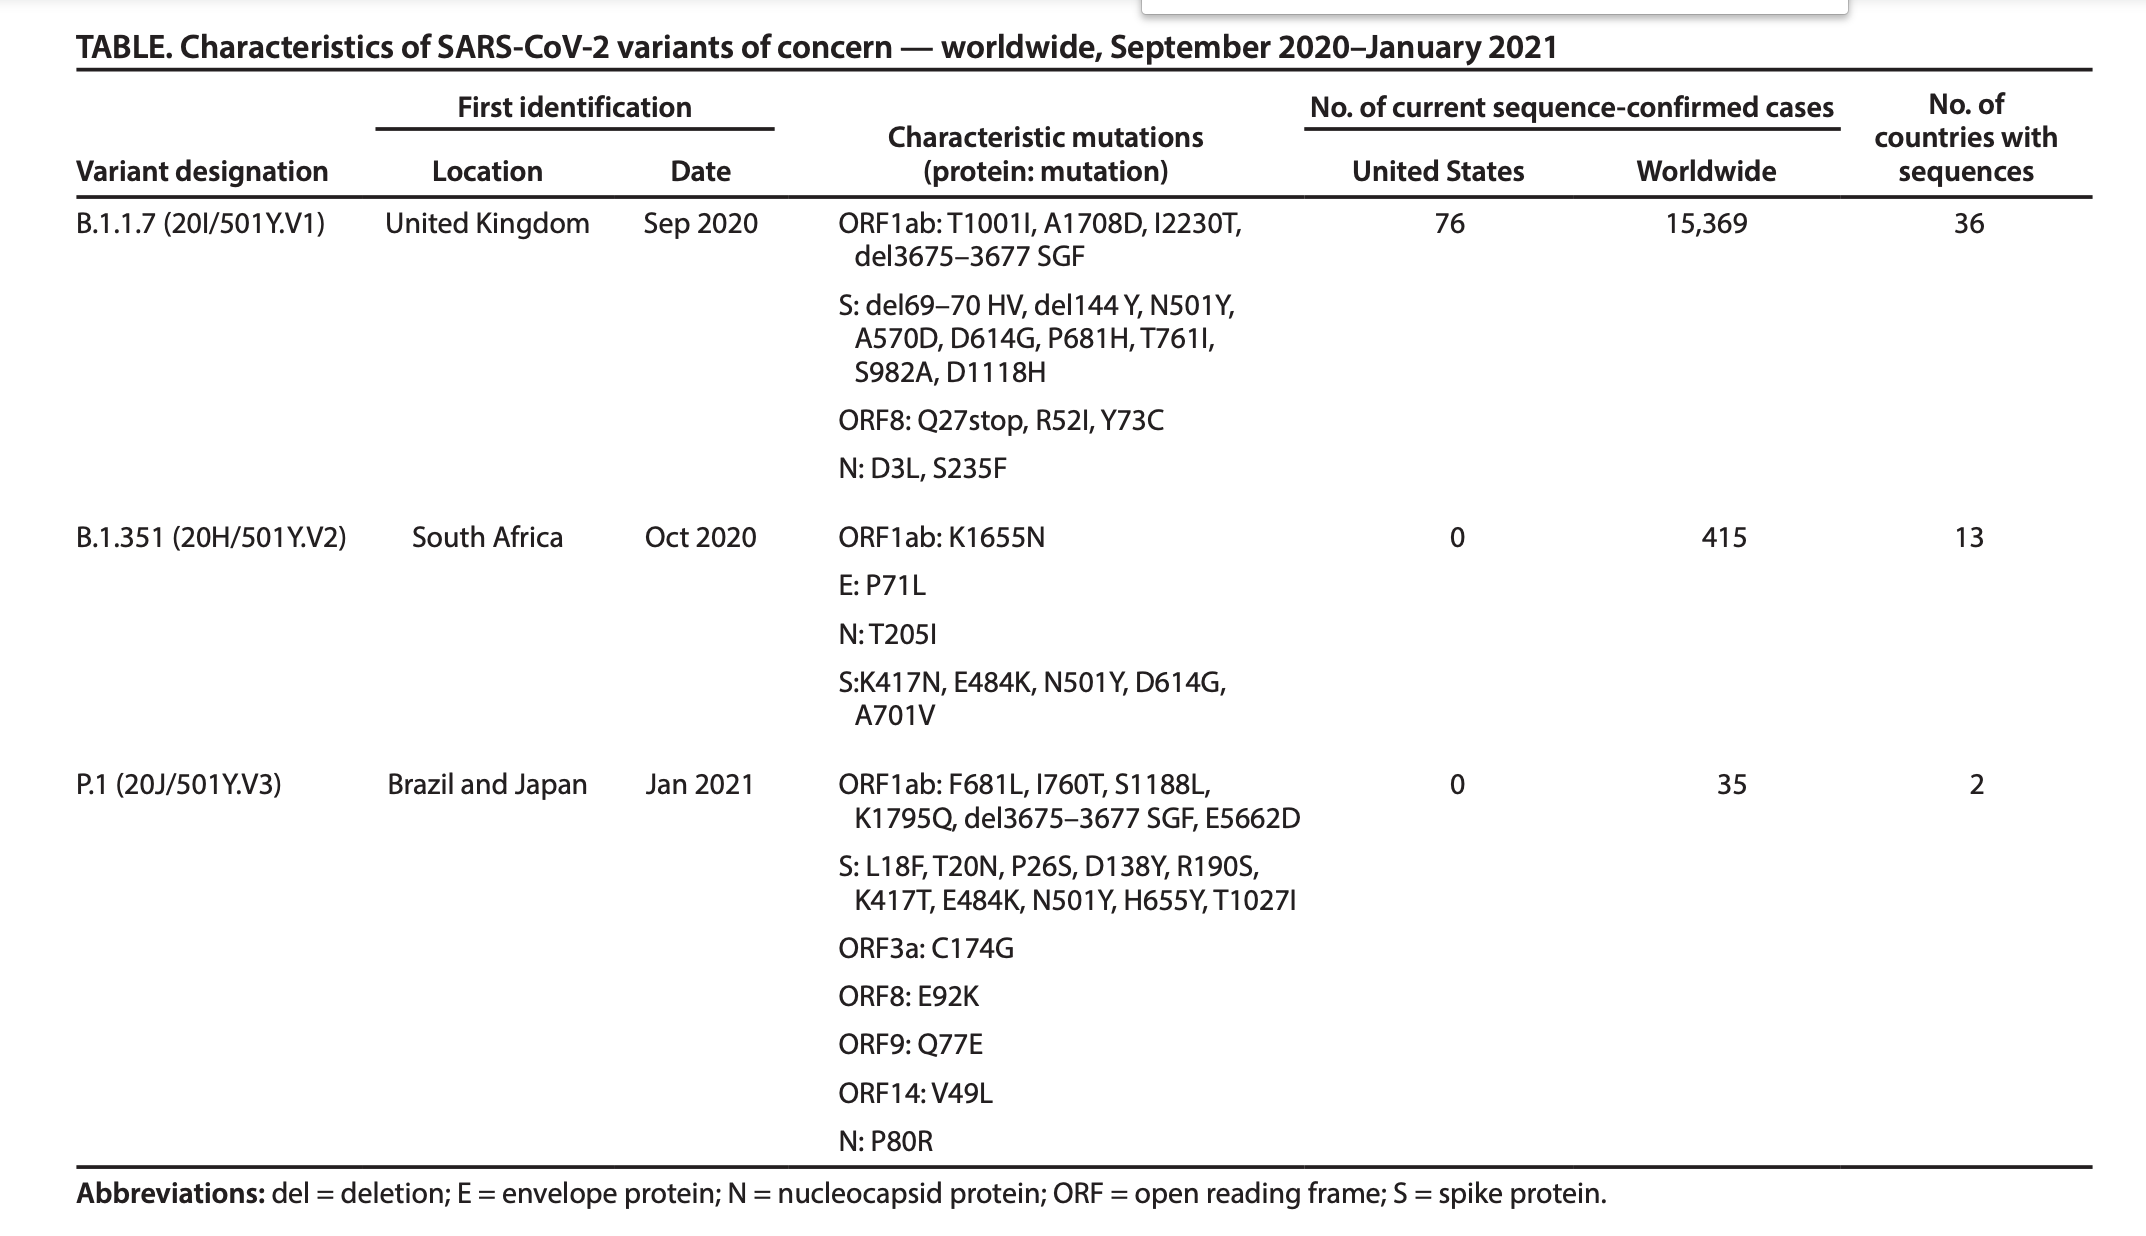
\includegraphics[scale=0.30] {images/cdc.png}}
\caption{Characteristics of SARS-CoV-2 variants of concern \cite{covid:cdc}}
\label{fig:cdc}
\end{figure}




\begin{figure} [H]
\center{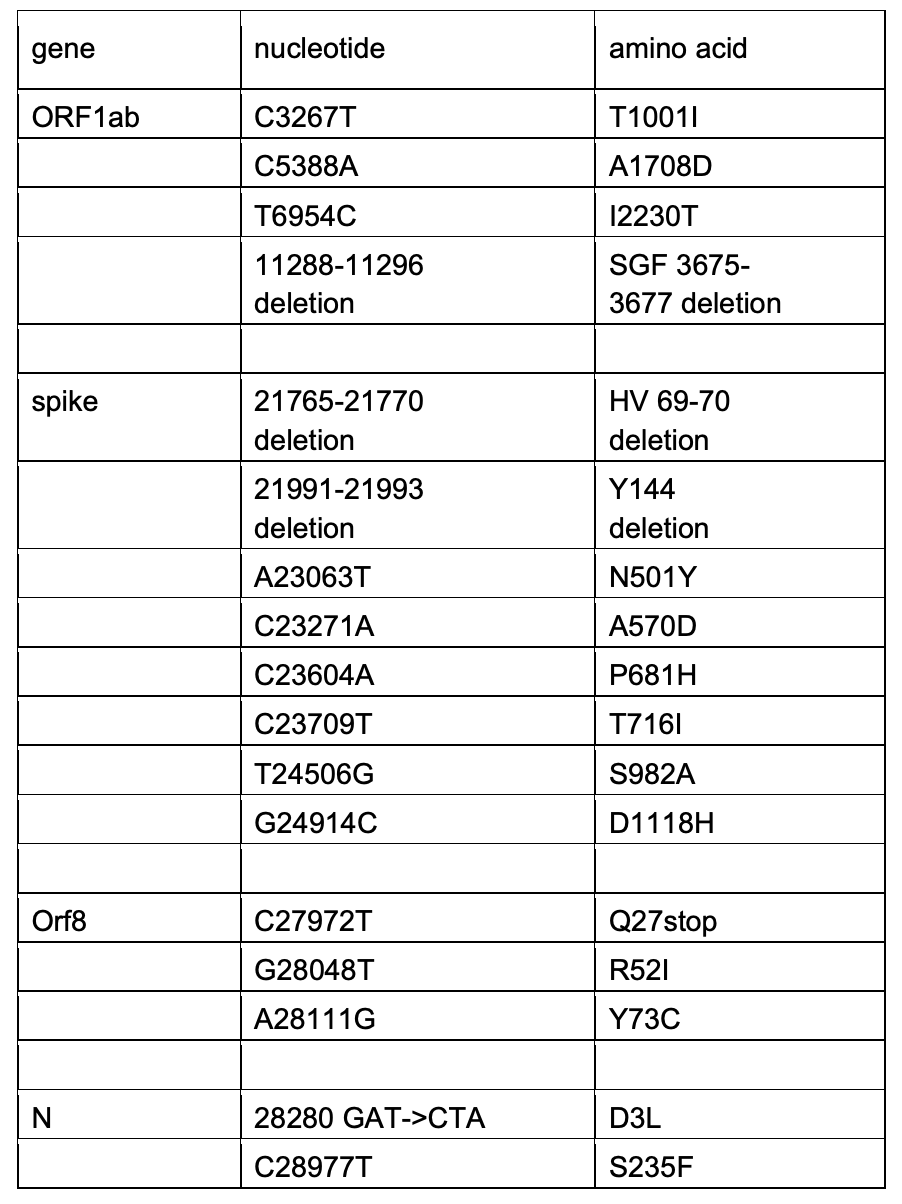
\includegraphics[scale=0.30] {images/b117_mutations.png}}
\caption{Protein altering mutations defining the B.1.1.7 variant \cite{covid:voc}}
\label{fig:b117_voc}
\end{figure}


\bibliographystyle{plain}
\bibliography{/Users/dmm/papers/bib/biology}


\end{document} 

